\documentclass{article}
\usepackage[utf8]{inputenc}

\usepackage{doobs}
\usepackage{mathpartir}
\usepackage{minted}
\usepackage{titlesec}
\usepackage{tcolorbox}

\usepackage{algorithm}
\usepackage{algpseudocode}

\DeclareUnicodeCharacter{3B4}{$\bm{\delta}$}
\DeclareUnicodeCharacter{3B8}{$\bm{\theta}$}
\DeclareUnicodeCharacter{3BB}{$\lambda$}
\DeclareUnicodeCharacter{3BC}{$\mu$}
\DeclareUnicodeCharacter{3BC}{$\pi$}
\DeclareUnicodeCharacter{3C3}{$\sigma$}
\DeclareUnicodeCharacter{3C0}{$\pi$}
\DeclareUnicodeCharacter{2200}{$\forall$}
\DeclareUnicodeCharacter{2203}{$\exists$}
\DeclareUnicodeCharacter{2208}{$\in$}
\DeclareUnicodeCharacter{2208}{$\in$}
\DeclareUnicodeCharacter{2260}{$\neq$}
\DeclareUnicodeCharacter{2227}{$\wedge$}
\DeclareUnicodeCharacter{2225}{$\|$}
\DeclareUnicodeCharacter{2194}{$\iff$}
\DeclareUnicodeCharacter{00AC}{$\neg$}
\DeclareUnicodeCharacter{2228}{$\vee$}
\DeclareUnicodeCharacter{2115}{$\mathbb{N}$}
\DeclareUnicodeCharacter{2124}{$\mathbb{Z}$}
\DeclareUnicodeCharacter{207A}{$^+$}
\DeclareUnicodeCharacter{2264}{$\leq$}
\DeclareUnicodeCharacter{2192}{$\to$}


\titleformat{\section}
  {\normalfont\Large\bfseries}{\thesection}{1em}{}[{\titlerule[0.3pt]}]

\begin{document}

\title{%
  Formal Verification of a Closest Pair Algorithm
  % \\
  % Final Project Report
  \\[0.5em]
  \large MIT 6.838 Final Project \\
}

\author{
Logan Weber\\
loganweb@mit.edu
}

\def\aSigma{\overline{\Sigma}}
\def\asigma{\overline{\sigma}}
\def\aheap{\overline{h}}

\date{}

\maketitle

\tableofcontents

% \section{TODOs}
Recall, Piotyr said what's most useful for him is statistics (breakdowns of code vs. proof) and ``war stories''.

Link to Github repo.

\section{Introduction}
In the past few years, the Lean theorem prover and programming language has caught the attention of the math community.
For a long time, proof assistants were thought of as unsatisfactory for formalizing undergraduate-level mathematics, let alone \textit{research}-level mathematics.
This image began to change when a challenge by Fields Medalist, Peter Scholze, was proposed: \href{https://xenaproject.wordpress.com/2020/12/05/liquid-tensor-experiment/}{The Liquid Tensor Experiment}.
This challenge involved formalizing a foundational result in a new area of mathematics.
The Lean community took up the challenge, and within 6 months, had formalized the most import aspects of the proof, far exceeding Scholze's expectations.

% No single innovation
The rise of Lean cannot be explained by any significant \textit{technological} innovation---it was a \textit{cultural} innovation.
% TODO this makes it sound like Lean isn't sound
The most relevant comparison is to the Coq proof assistant, which has emphasized sound, type-theoretic principles since its conception.
Lean instead focuses on directly accomodating the workflows of mathematicians, embracing language features that elude type-theoretic grounding (e.g., quotients) and that destroy computational properties (e.g., the law of excluded middle).

Because of Lean's focus on ergonomics, it has attracted a number of mathematicians, who have formalized a substantial body of undergraduate-level mathematics in a library known as \href{https://leanprover-community.github.io}{Mathlib}.

% As a result, Lean encourages the use of classical logic.
% A notable point of contrast that arises from this stated goal is that classical logic (i.e., using the law of excluded middle)
% As a result, Lean has incorporated quotient types and embraces classical mathematics, which uses the law of excluded middle, destroying computational properties.
% With that being said.


% TODO doesn't seem like this is true after reading into it. seems more like the emphasis on the axiom of choice and baked-in quotient types was important.
% It was a plethora of performance engineering and ergonomic improvements that made Lean an attractive platform for the formalization of mathematics.

Earlier this term, Professor Indyk mentioned the difficulties a past student had when verifying one of the algorithms from lecture.
In this project, my goal is to survey the state of formal verification as it pertains to geometric computing.
The question I seek to answer is: how much of the proof burden does Mathlib alleviate in the process of formal verification?

% In an earlier lecture this term, a student asked Professor Indyk how some of the algorithm analysis we had done could be made formal.
% He replied with an anecdote that a student once tried to formally verify an algorithm in his class.
% The author took this as a challenge and decided to assess the current state of formal verification, given the existence of libraries like Mathlib.

The concrete goal I set out with on this project was to implement and formally verify the closest pair (with help) and helper finder algorithms.

My background is not in formal verification, but I do have a background in programming languages broadly.
As someone who has been skeptical of the efficacy of verification, part of my goal with this project is to give perspective to outsiders and tell them what they should expect, without sugar-coating it and saying ``you'll get used to it''.

Our final achievements were
\footnote{
  Code can be found at \href{https://github.com/weberlo/verified-gridding}{https://github.com/weberlo/verified-gridding}.
}:
\todo{Make it like a TODO list with checkmarks on things we completed}
\begin{itemize}
  \item An implementation for a restricted form of the closest pair (with help) problem.
  \item A ``broad strokes'' verification of the algorithm, with many low-level lemmas assumed to be true.
\end{itemize}

\todo{Do some fenceposting}

\section{Background}
In this section, we recap the closest pair with help problem and the algorithm presented in class that solves it (\shortref{sec:cp_with_help}).
Then, we cover simplifications and restrictions we imposed on the specification, to make it amenable to formal verification (\shortref{sec:cp_with_help_simple}).
Finally, we collect all notation used in this report and motivate the nonstandard notation (\shortref{sec:notation}).
\todo{Fencepost}

\subsection{Closest Pair With Help}\label{sec:cp_with_help}
Recall the problem specification for closest pair (with help) below.

\begin{tcbproblem}{\sc{Closest Pair With Help}}{}
  Given a set of points $P \subseteq \R^d$, find the closest pair
  \[ (p^*, q^*) = \argmin_{(p,q) \in P\times P, p\neq q} \|p - q\|_2, \]
  knowing $\|p^* - q^*\|_2 \in (t, ct]$.
\end{tcbproblem}

The algorithm we saw in Lecture 11 to solve this problem is as follows.
\begin{algorithm}
  \caption{Closest Pair With Help}\label{alg:cp_with_help}
  \begin{algorithmic}
  \State $g \gets $ grid with side lengths $k = 1/\sqrt{d}$.
  \State Insert each point $p$ in the bucket in $g$ with index $\lfloor p / k \rfloor$.
  \State $x\!y \gets \mathsf{none}$
  \For{$p \in P$}
    \For{$\vec{v} \in [-\lceil c + 1 \rceil, \lceil c + 1 \rceil]^d$}
      \State $x\!y \gets \argmin \{ x\!y, \argmin_{q \in g[\lfloor p+\vec{v} / k \rfloor]}\{\| p - q \|\}\}$
    \EndFor
  \EndFor
  \State \Return $x\!y$
  \end{algorithmic}
\end{algorithm}

\subsection{Simplified Closest Pair With Help}\label{sec:cp_with_help_simple}
For the sake of both simplicity and computability, we impose the following restrictions on the specification in Section~\ref{sec:cp_with_help}:
\begin{itemize}
  \item \textbf{The points have integral components.} Lean does not include facilities for computing with real numbers, though, in principle, it could---with all results computed up to \textit{finite} precision.
  Without such facilities, we are left with $\Q$ or $\Z$ as natural carrier types.
  We chose $\Z$, believing it would be simpler.
  In hindsight, using $\Q$ may have been just as easy and perhaps easier.
  Since $\Q$ forms a field, it has multiplicative inverses, which simplifies algebra.
  \item \textbf{The points are in the plane.} This assumption was for simplicity on the first pass through the verification.
  We now believe generalizing to arbitrary dimension would require nontrivial changes in the implementation and the proofs.
  \todo{Would it tho?}
  \item \textbf{The norm is the \textit{squared} Euclidean norm.}
  We're working with integers and the outermost operation of $\| \cdot \|_2$ is a square root, which could return a value outside of $\Z$.
  Our fix is to consider the squared Euclidean norm $\| \cdot \|_2^2$.
  \item \textbf{The points are scaled so $t=1$.}
  We assumed this property in class, but because we're working with integers, it's a stronger assumption; scaling down could lose information and cause us to return the wrong pair.
\end{itemize}
With these restrictions, the specification now looks like the following, with changes highlighted in blue.
\begin{tcbproblem}{\sc{Closest Pair With Help (Restricted)}}{}
  Given a set of points $P \subseteq {\color{blue}\Z^2}$, find the closest pair
  \[ (p^*, q^*) = \argmin_{(p,q) \in P\times P, p\neq q} {\color{blue}\|p - q\|_2^2}, \]
  knowing $\|p^* - q^*\|_2^2 \in {\color{blue}(1, c]}$.
\end{tcbproblem}

\todo{Recap the algorithm.}

\paragraph{Trivial Grids.}
A notable corollary of these restrictions is that the mapping from points to their grid indices is the identity map.
Recall, we wish to set the grid size $k$ so the diameter of each cell is $< 1$, guaranteeing at most one point per cell.
We assume the bottom and left cell edges are inclusive and the top and right edges are exclusive.
Then, the furthest integer point from the bottom left $(0, 0)$ is at $(k - 1, k - 1)$.
\begin{align*}
  \| (k - 1, k-1) \|_2^2 & < 1 \\
  2(k-1)^2 & < 1
\end{align*}
The only integral solution is 1, so each point's grid index is itself.

\paragraph{Different Search Bounds.}
Knowing the closest pair distance is at most $c$, our norm gives us bounds on how many cells away we must search.
If $\| p^* - q^* \| \leq c$, then $(p_1^* - q_1^*)^2 + (p_2^* - q_2^*)^2 \leq c$, meaning $(p_1^* - q_1^*)^2\leq c$ and $(p_2^* - q_2^*)^2 \leq c$.
Then for each component $a$ of $p$ and $b$ of $q$, we have
\begin{align*}
  (a - b)^2 & \leq c \\
  |a - b| & \leq \sqrt{c}^\N
\end{align*}
where $\sqrt{n}^\N$ is the largest number $k$ such that $k^2 \leq n$.
So if we search hypercubes of radius $\sqrt{c}^\N + 1$, we will certainly find the closest pair.

\paragraph{The Simplified Algorithm.}
With this simplified specification and the observations above, we verify the following modified algorithm (again, with changes highlighted in blue).

\begin{algorithm}
  \caption{Simplified Closest Pair With Help}\label{alg:cp_with_help_simple}
  \begin{algorithmic}
  \State $g \gets $ grid with side lengths ${\color{blue}k = 1}$.
  \State Insert each point $p$ in the bucket in $g$ with index $\color{blue}p$.
  \State $x\!y \gets \mathsf{none}$
  \For{$p \in P$}
    \For{$\vec{v} \in {\color{blue}[-(\sqrt{c}^\N + 1), \sqrt{c}^\N + 1]^2}$}
      \State $x\!y \gets \argmin \{ x\!y, \argmin_{q \in {\color{blue}g[p+\vec{v}]}}\{\| p - q \|\}\}$
    \EndFor
  \EndFor
  \State \Return $x\!y$
  \end{algorithmic}
\end{algorithm}

\todo{Include diagram from presentation?}
\todo{Add a section somewhere discussing how we might tackle the problem of removing these assumptions}

% \begin{minted}{lean}
% def closest_pair (p q : point) (ps : list point) : Prop :=
%   (p ∈ ps) ∧ (q ∈ ps) ∧ (p ≠ q) ∧
%   (∀ (r s : point), r ≠ s → ∥p - q∥ ≤ ∥r - s∥)

% def closest_pair_with_help (p q : point) (ps : list point) (c : ℕ⁺) : Prop :=
%   (closest_pair p q ps) ∧ (1 < ∥ p - q ∥) ∧ (∥ p - q ∥ ≤ c)
% \end{minted}
% \newpage

\subsection{Notation}\label{sec:notation}
Here, we explain any notation in Table~\ref{fig:notation_summary} that was not explained in the previous subsections and that will be useful in later sections.
\todo{Double back after the fact and check which symbols we actually need for points}
\begin{figure}[H]
\begin{center}\label{fig:notation_summary}
\begin{tabular} {|| r | l ||}
  \hline
  Notation & Description \\
  \hline
  \hline
  $P \subseteq \Z^2$ & list of input points to the algorithm \\
  \hline
  $P' \subseteq P$ & proposition that $P'$ is a sublist of $P$ \\
  \hline
  $[]$ & the empty list \\
  \hline
  $p :: P'$ & the list $P'$ with $p$ appended to the front \\
  \hline
  $p, q, r, s, x, y, z, w \in P$ & points in $P$ \\
  \hline
  $a, b \in \Z$ & integers \\
  \hline
  $k, m, n \in \N$ & natural numbers \\
  \hline
  $c \in \N^+$ & the distance hint \\
  \hline
  $(P \times P)^?$ & set of potentially null point pairs in $P$ \\
  \hline
  $x\!y, z\!w, r\!s \in (P \times P)^?$ & potentially null pairs of points in $P$ \\
  \hline
  $\mathsf{some}(x, y) \in (P \times P)^?$ & definitely non-null pairs of points in $P$ \\
  \hline
  $\mathsf{none} \in (P \times P)^?$ & definitely null pairs of points in $P$ \\
  \hline
  $x\!y \leq z\!w$ & proposition that the \textit{nullable} pair $x\!y$ \\ & is closer together than $z\!w$ \\
  \hline
  $\text{CP}_P(x, y)$ & $(x, y)$ is the closest pair in $P$ \\
  % \coloneqq (x, y) = \argmin_{(p, q) \in P} \| p - q \|$ & $(x, y)
  \hline
  $B(p, c)$ & set of points $\in \Z^2$ within distance $c$ of the point $p$ \\
  \hline
  $B_P(p, c)$ & set of points $\in P$ within distance $c$ \\ & of the point $p$ (i.e., $B(p, c) \cap P$) \\
  \hline
  $\widetilde{\text{CP}}_P(x\!y)$ & $x\!y$ is the closest pair in $\bigcup_{p \in P} \left(p, B_P(p, c)\right)$, \\ & or $\mathsf{none}$ if there are no pairs in this set \\
  \hline
  $\mathsf{Grid} \coloneqq (\mathsf{grid} : \Z^2 \rightharpoonup [\Z^2]) \times$ & the type/fields of our grid structure \\
  $(P : [\Z^2]) \times$ & \\
  $(c : \N^+){\color{white}\times}$ & \\
  \hline
  $G(P, c) : \mathsf{Grid}$ & grid constructed from set of points $P$ \\
  & and distance hint $c$ \\
  \hline
  $g : \mathsf{Grid}$ & arbitrary grid structure \\
  \hline
  $g[p]$ & points in cell at index $p$ \\
  \hline
  $\| \cdot \|$ & the \textit{squared} Euclidean norm \\
  \hline
  $\sqrt{n}^\N$ & the natural number square root \\
  \hline
  $\lfloor p \rfloor$ & pointwise application of floor function to $p$ \\
  \hline
\end{tabular}
\end{center}
\caption{Summary of notation used throughout our report}
\end{figure}
\todo{Could clean this table up with multitable maybe?}
\todo{Should we use list notation for G(P, c)?}
\todo{Swap argument order of $G$ to $G(P, c)$}
\todo{Add list cons notation, list subset notation, and $l$ for a list and $L$ for a list of lists}
\todo{Mark lemmas that should exist in Mathlib as blue in the diagram}
\todo{Use $g[p]$ notation in algorithm environment}

Most of our notation is standard or self-explanatory, so we focus on motivating the outliers.

\paragraph{Potentially null point pairs.}
Because the algorithm searches for pairs within balls around points, we must account for the case where there are no such pairs.
We handle this outcome by lifting the type of point pairs $(P \times P)$ to the type $(P \times P)^?$ of possibly null point pairs.
This type has inhabitants of the form $\mathsf{none}$, expressing a null pair, and $\mathsf{some}(x, y)$, expressing a non-null pair.
When we have a term of type $(P \times P)^?$, and we don't yet know whether it's null, we write it as $x\!y$.

% In accordance with functional programming convention, we express a pair of points being null with the term $\mathsf{none}$, and we express non-null pairs of points $(x, y)$ with the term $\mathsf{some}(x, y)$.

\paragraph{Ordering on potentially null point pairs.}
In the algorithm, we frequently compare a single ball's closest pair to the closest pair from a lower recursion level.
Both of these results could be null, so we must case on whether zero, one, or both are null and choose the ``closest'' result accordingly.

Instead of littering our code with casework on nullable pairs, we impose an order $x\!y \leq z\!w$ on $(P \times P)^?$, with $\mathsf{none}$ representing a pair that is infinitely distant.
Our order satisfies the following rules:
\begin{align*}
  \mathsf{none} & \leq \mathsf{none} \\
  \mathsf{none} & \not\leq \mathsf{some}(z, w) \\
  \mathsf{some}(x, y) & \leq \mathsf{none} \\
  (\mathsf{some}(x, y) \leq \mathsf{some}(z, w)) &\Leftrightarrow (\|x - y\| \leq \|z - w\|)
\end{align*}

\paragraph{Ball of points in $P$.}
Conceptually, our algorithm draws balls around points in $P$ and finds other points in $P$ lying within those balls.
To express this concept in our proofs, we augment standard $B(p, c)$ notation to $B_{P}(p, c) \coloneqq B(p, c) \cap P$, which includes all points in $P$ lying within $B(p, c)$.

\paragraph{Closest pair in union of balls.}
As we will see in Section~\ref{sec:change_ih}, directly proving the $(x, y)$ returned by our algorithm is the closest pair (i.e., $\text{CP}_P(x, y)$) doesn't work.
Instead, we define a predicate $\widetilde{\text{CP}}_P(x\!y)$, expressing that $x\!y$ is the closest pair among all pairs in balls we draw around points in $P$.
Then, we prove our algorithm satisfies this predicate.

\paragraph{Grid construction.}
We require a few lemmas expressing properties about the grid structure, so we notate it as a tuple $G(P, c)$ with fields
\begin{itemize}
  \item $(\mathsf{grid} : \Z^2 \rightharpoonup [\Z^2])$: the hash table mapping grid indices to cells containing lists of points.
  \item $(P : [\Z^2])$: the set of points used to generate the grid.
  We need to carry this data around to express relations between the set of input points and the $\mathsf{grid}$ we create.
  \item $(c : \N^+)$: the distance hint.
  We include this for similar reasons to why we include $P$.
\end{itemize}
When we don't have access to the parameters a grid was constructed with, we notate it as $g$.

% \begin{minted}{lean}
% def find_closest_pair (ps : list point) (c : ℕ⁺) : (point × point) := sorry

% theorem find_closest_pair_correct :
%   ∀ (ps : list point) (c : ℕ⁺),
%     (∃ (p q : point),
%       (closest_pair p q ps) ∧ (1 < ∥ p - q ∥) ∧ (∥ p - q ∥ ≤ c)) →
%     (∃ (p q : point),
%       find_closest_pair ps c = (p, q) ∧
%       closest_pair p q ps) := begin
%   sorry
% end
% \end{minted}

% \section{Implementation}
% We won't waste much breath on the implementation.

\section{Verification}
\todo{Give top-down proof strategy spiel}

\subsection{Code Structure}
\todo{Try to assign mathematical notation to each of these}
\begin{center}
\begin{tabular} {|| r | l | p{5cm} ||}
  \hline
  Function Name & Signature & Description \\
  \hline
  \hline
  \texttt{find\_closest\_pair} &
  $(c : \N^+) \to (P : [\Z^2]) \to (P \times P)^?$ &
  The entry point to our algorithm.
  Constructs the grid, then calls \texttt{aux}.
  If the result is further than distance $c$, returns $\mathsf{none}$. \\
  \hline
  \texttt{aux} &
  $(g : \mathsf{Grid}) \to (P : [\Z^2]) \to (P \times P)^?$ &
  The core subroutine of the algorithm.
  Recurses over $P$, using \texttt{mdp\_with} at each point $p$ to find points in $B_{P}(p, c)$.
  \\
  \hline
  \texttt{grid\_points} &
  $(P : [\Z^2]) \to (c : \N^+) \to \mathsf{Grid}$ &
  Creates the grid structure, inserting points according to \texttt{get\_grid\_idx}. \\
  \hline
  \texttt{min\_dist\_pair} &
  $(p : \Z^2) \to (Q : [\Z^2]) \to (P \times P)^?$ &
  Given $p$ and a list of points in a ball around it, returns the closest point to $p$.  \\
  \hline
  \texttt{mdp\_with} &
  $(p : \Z^2) \to (g : \mathsf{Grid}) \to (P \times P)^?$ &
  Collects points around $p$ via \texttt{get\_neighbs}, then uses \texttt{min\_dist\_pair} to find the closest among them.
  \\
  \hline
  \texttt{get\_grid\_idx} &
  $(p : \Z^2) \to \Z^2$ &
  \\
  \hline
  \texttt{get\_hypercube} &
  $(n : \N) \to [\Z^2]$ &
  \\
  \hline
  \texttt{get\_idxs} &
  $(p : \Z^2) \to (c : \N^+) \to [\Z^2]$ &
  \\
  \hline
  \texttt{lift\_option\_list} &
  $\forall (\alpha : \mathsf{Type}).\, [\alpha]^? \to [\alpha]$
  &
  \\
  \hline
  \texttt{get\_neighbs} &
  $(p : \Z^2) \to (g : \mathsf{Grid}) \to [\Z^2]$ &
  \\
  \hline
\end{tabular}
\end{center}


The goal of our verification is to prove the following theorem.
\begin{tcbtheorem}{{\large\texttt{find\_closest\_pair}} Finds Closest Pair}{main_finds_cp}
If the closest pair is within distance $(1, c]$, \texttt{find\_closest\_pair} finds $(x, y)$ such that $\text{CP}_P(x, y)$.
\end{tcbtheorem}

\todo{Somehow mark the goal lemma about find closest pair in the figure.  Can't bold it because we're already bolding the lemmas of interest.  Maybe a star?  Or big letters saying "GOAL"}
\begin{figure}[H]
  \begin{center}
  \includegraphics[width=\linewidth]{res/proof_dependency}
  \end{center}
  \caption{
    Graph capturing the dependency of each lemma/theorem on other lemmas.
    An edge exists from $a$ to $b$ when $a$ is used by $b$ (e.g., a lemma with high in-degree uses many lemmas).
    A dashed border means the lemma has not been proven.
    A bold border means the lemma is important/interesting/difficult, and we cover it in Section~\ref{sec:war_stories}.
  }
\end{figure}


\subsection{Predicates}
\begin{center}
\begin{tabular} {|| c | c | c ||}
  \hline
  Predicate Name & Signature & Description \\
  \hline
  \hline
  \texttt{pt\_in\_ball} & & \\
  \hline
  \texttt{closest\_pair} & & \\
  \hline
  \texttt{cp\_with\_help} & & \\
  \hline
  \texttt{closest\_pair\_in\_ball\_union} & & \\
  \hline
  \texttt{in\_opt\_list} & & \\
  \hline
  % \hline
\end{tabular}
\end{center}

% \begin{minted}{lean}
% inductive closest_pair_in_balls (c : ℕ⁺) (qs : list point) :
%   option (point × point) → list point → Prop
% | no_ball (xy : option (point × point)) : closest_pair_in_balls xy []
% | succ_ball (xy : option (point × point)) (p : point) (ps' : list point) :
%     ((∃ (q : point), q ∈ qs ∧ ∥q - p∥ ≤ c) →
%       ∃ (x y : point),
%         xy = some (x, y) ∧
%         (∀ (q : point),
%             q ∈ qs →
%             ∥q - p∥ ≤ c →
%             ∥x - y∥ ≤ ∥q - p∥)) →
%     closest_pair_in_balls xy ps' →
%     closest_pair_in_balls xy (p :: ps')
% \end{minted}

\subsection{War Stories}\label{sec:war_stories}
In this section, we cover proofs which were either conceptually interesting or highlight some of the difficulties of working with Lean.

\subsubsection{{\large\texttt{aux}} Finds the Closest Pair (in the Union of Balls)}\label{sec:change_ih}

As mentioned in Section~\ref{sec:idk_where}, \texttt{aux} is a recursive function that performs the core iteration over the list of points $P$---\texttt{find\_closest\_pair} simply creates the grid and filters the result of \texttt{aux} if it's not within distance $c$.
Thus, the most important property to prove is that \texttt{aux} finds the closest pair, given that the distance hint holds true.

\begin{tcblemma}{{\large\texttt{aux}} Finds Closest Pair}{aux_finds_cp}
If the closest pair is within distance $(1, c]$, \texttt{aux} finds $(x, y)$ such that $\text{CP}_P(x, y)$.
\end{tcblemma}

When you prove facts about a recursive function, you often prove them by induction.
If we want to prove our algorithm finds the closest pair, a naive induction on $P$ would have us prove the following in the induction step:
\begin{quote}
  Suppose we know the recursive subcall on the sublist $P'$ gives us the closest pair in $P'$.
  Then the current call gives us the closest pair for the larger list $P = p :: P'$.
\end{quote}
But the antecedent doesn't hold for our algorithm.
In particular, the closest pair might contain points we haven't recursed over yet.
We can see the issue in step 3 of Figure~\ref{fig:aux_invariant} (right).
The closest pair at this step includes a point outside the list of processed points, identifying a case where the naive invariant fails.
\begin{figure}[H]\label{fig:aux_invariant}
  \begin{center}
  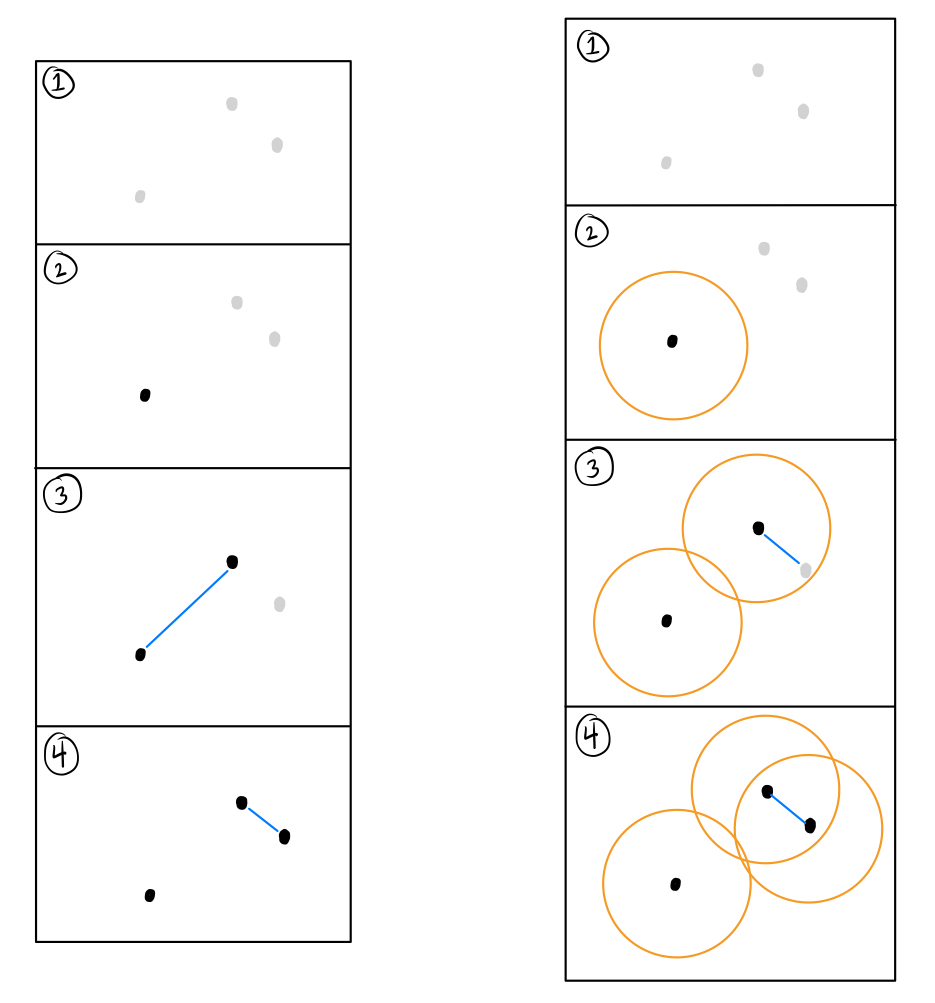
\includegraphics[width=0.5\linewidth]{res/aux_invariant}
  \end{center}
  \caption{
    Depiction of the pairs satisfying the inductive hypothesis at each step of the algorithm, for both the naive and correct invariants.
    Black dots represent points in $P' \subseteq P$ that have been processed and gray dots represent unprocessed points in $P$.
    \textbf{(Left)}
      Pairs satisfying the naive induction invariant, expressing that the algorithm maintains the closest pair in $P'$.
    \textbf{(Right)}
      Pairs satisfying the correct induction invariant, expressing that the algorithm maintains the closest pair in $\bigcup_{p \in P'}B_P(p, c)$.
  }
\end{figure}
We need a proof goal that provides us with a different, stronger induction hypothesis.
Our algorithm, conceptually speaking, draws balls around each point and finds the closest pair among all balls seen so far.
To capture this process in a predicate, we create a recursively defined predicate $\widetilde{\text{CP}}_P(x\!y)$ satisfying the following rules:
\begin{itemize}
  \item \textbf{No points:} $\widetilde{\text{CP}}_P(\mathsf{none}, [])$
  \label{case:rec_pt_closer}
  \item \textbf{Recursive point closer:} If $\widetilde{\text{CP}}_P(x\!y, P')$ and $x\!y$ is closer than all points in $B_P(p, c)$, then $\widetilde{\text{CP}}_P(x\!y, p :: P')$.
  \label{case:curr_pt_closer}
  \item \textbf{Current point closer:} If $\widetilde{\text{CP}}_P(x\!y, P')$, but there is a point $q \in B_P(p, c)$ closer to $p$ than any other point in $B_P(p, c)$, and $(p, q)$ is closer than $x\!y$, then $\widetilde{\text{CP}}_P(\mathsf{some(p, q)}, p :: P')$.
\end{itemize}
Now, instead of proving \texttt{aux} finds $(x, y)$ such that $\text{CP}_P(x, y)$, we prove the following.

\begin{tcblemma}{{\large\texttt{aux}} Finds Closest Pair in Ball Union}{aux_finds_cp_in_ball_union}
\texttt{aux} finds $(x, y)$ such that $\widetilde{\text{CP}}_P(\mathsf{some}(x, y))$.
\end{tcblemma}
This lemma provides the correct induction hypothesis, allowing the proof to go through.

With Lemma~\ref{lem:aux_finds_cp_in_ball_union} proven, we still need to prove Lemma~\ref{lem:aux_finds_cp}.
To do so, we prove the lemma below, which combines Lemma~\ref{lem:aux_finds_cp_in_ball_union} with the distance hint.
For brevity, we omit discussion of the proof, though we discuss one of the lemmas it relies on in Section~\ref{sec:cp_in_ball_union_high_level}.

\begin{tcblemma}{($\widetilde{\text{CP}}_P$ and Distance Hint) $\Rightarrow$ $\text{CP}_P$}{cp_in_ball_union_and_distance_hint}
\texttt{aux} finds $(x, y)$ such that $\widetilde{\text{CP}}_P(\mathsf{some}(x, y))$.
\end{tcblemma}

% \todo{Import graphic from presentation}
% This one is interesting because it highlights the concept of strengthening (or rather, ``aligning'') the induction hypothesis.

% Our core algorithm recurses on the list of points, combining results from subcalls to eventually arrive at the closest pair.
% Then it seems natural for our proof of the algorithm's correctness to mirror its definition, which we could achieve by inducting on the list of points.

% However, inducting on the list of points to prove the closest pair predicate gives us an incorrect induction hypothesis.
% The induction hypothesis will state that the recursive call contains the closest pair among all of the points processed in the recursive call.
% But this is not true!
% Since we draw balls around each point that we process, we may pick points outside of the set of points we have recursed over.

% Thus, we must strengthen the induction hypothesis to more closely align our analysis of the algorithm than the definition.


\subsubsection{Closest Pair In Ball Union Closer Than All Points Within Distance $\mathbf{c}$}
\label{sec:cp_in_ball_union_high_level}
In proving Lemma~\ref{lem:cp_in_ball_union_and_distance_hint}, we require the following lemma.
\begin{tcblemma}{$\widetilde{\text{CP}}_P$ Flattening}{}
  If $\widetilde{\text{CP}}_P(\mathsf{some}(x, y))$ and $q \in \bigcup_{p \in P} B_P(p, c)$, then $(x, y)$ is closer than $(p, q)$.
\end{tcblemma}
After staring for a bit, you might think this lemma should hold trivially\footnote{
  The reader may be thinking this of many results in this report... and they are not alone.
  Such is life in formal verification, it seems.
}.
After all, isn't this exactly what $\widetilde{\text{CP}}_P$ is meant to express?
Indeed it is, but the proof of this fact is not automatic.
The reason is that $\widetilde{\text{CP}}_P$ is more specific than the simpler statement of being the closest pair in $\bigcup_{p \in P} B_P(p, c)$, because it enforces a particular \textit{process} by which the closest pair was arrived at.
This process is recursive, so to arrive at the ``flattened'' proposition above, we need to ``unroll'' it via induction.
But induction on what?

We may wish to induct on the list of points $P$, but this causes an issue in the case where the current point is closer (see \ref{case:curr_pt_closer}).
Since we're inducting on $P$, all other variables remain fixed in the induction hypothesis.
So if we're trying to prove that $(x,y)$ is closer than $(p,q)$ and we want to apply the induction hypothesis, we need to provide a proof that $(x, y)$ satisfies $\widetilde{\text{CP}}_{P'}(\mathsf{some}(x, y))$.
However, in the case where the current point is closer, we have that some other point pair $x\!y'$ was the closest pair in the ball union for the sublist $P'$.
Thus, we only have $\widetilde{\text{CP}}_{P'}(x\!y')$, and we are unable to apply the IH.

The issue is that inducting on $P$ leaves $(x, y)$ fixed and does not account for the fact that the closest pair changes as we recurse.
What else can we induct on then?
Well, induction can be performed on any type satisfying certain conditions\footnote{In particular, we must be able to impose a \textbf{\textit{well-founded order}} upon it.}, and it so happens that our recursive predicate $\widetilde{\text{CP}}$ satisfies them.
This induction target solves our problem because the inductive hypothesis changes depending on whether we are in the case where the recursive result remains the closest or a pair in the current point's ball is closer.

There are two takeaways from this proof:
\begin{itemize}
  \item In verification, you often define predicates that are aligned with the recursion structure of an algorithm, for the reasons outlined in Section~\ref{sec:change_ih}.
  However, this often leads to an abstraction mismatch, because these predicates don't directly encode high-level mathematical properties.
  Thus, it is common to prove lemmas that lift these low-level predicates to intuitive statements you can work with in other proofs.
  \item Induction on recursively defined predicates can yield stronger induction hypotheses or, at least, hypotheses that are more closely aligned with the proof goal.
\end{itemize}
\todo{Update CP instances in diagram to have P subscript}

% \paragraph{Induction on Recursively Generated Propositions.}
% When you have a recursively defined proposition, sometimes induction on a single index (think of it like a variable) doesn't give the right induction hypothesis.
% For example, when proving that the closest pair in the ball union is the closest pair among all points in the ball union \todo{need to go to the level of logic to make this statement not sound trivial}, inducting on the list of points we recurse over gives an unhelpful induction hypothesis in the case where we update the pair.
% This is because the pair is held fixed throughout the induction (we're only inducting over the point list), but the pair changes in the algorithm when we encounter a closer pair.
% To achieve the correct IH, we induct on the $\text{CP}_P{\mathcal{B}(\mathsf{ps}, c)}(xy)$ proposition itself.
% After all, we defined it recursively, so structural induction applies equally well to it.
% Because we vary multiple parameters in some cases of the proposition, this induction structure is aligned with the process and gives us the proper IH in the update case.

% In general, if you have \textit{multiple} arguments that change throughout the algorithm, induction on any single argument will only capture the variance in one of the parameters.
% Induction on the structure of the proposition.

% \paragraph{Side Note.} It seems intuitive that the predicate we've been calling ``the closest pair in the ball union'' should satisfy the property that any pair within distance $c$ will be at least as far away as the closest pair in the ball union.

% You could argue then that we've been using the wrong terminology for the recursively defined predicate.
% This lemma about the predicate is the property we desired all along and the predicate is somehow lower level than this property, and it shows more than just the property, but rather a \textit{process} we use to arrive at the property.

% This sheds some light on what we've done mathematically.
% We've taken the closest pair predicate and refactored it into the distance hint and the lemma that we find the closest pair within the ball union.
% The inductive predicate we define is a means of elaborating on the latter property so that its recursion structure is aligned with that of our algorithm.

\subsubsection{Bounded Norm $\Rightarrow$ In $\ell_\infty$ Ball}
On the path to proving Lemma~\ref{lem:aux_finds_cp_in_ball_union}, we need lemmas showing that we check the correct grid indices.
The lemma below says that if the distance between two points is bounded, then checking in a hypercube of a certain radius around one of them suffices to find one of the points.
\begin{tcblemma}{Hypercube Containment for Bounded Norm}{}
  If $\|(a, b)\| \leq c$, then $(a, b) \in \texttt{get\_hypercube}(\sqrt{c}^\N + 1)$.
\end{tcblemma}
There's nothing conceptually tricky about this lemma.
However, it turned out to be an absolute pain to prove in Lean.

We first break down the proof goal with a lemma showing it suffices to prove
\[ -\coerce{\sqrt{c}^\N + 1}{\Z} \leq a, b \leq \coerce{\sqrt{c}^\N + 1}{\Z}. \]
Recall, $\coerce{n}{\Z}$ represents a coercion of $n \in \N$ into an integer.
This coercion is a trivial inclusion, but we were unable to convince Lean of this simple fact.

We now focus on just $-\coerce{\sqrt{c}^\N + 1}{\Z} \leq a$.
The other cases are similar.

 one side of the inequalities and just one of the variables

We then proceed by contradiction, giving us the hypothesis that
$\neg(-\coerce{\sqrt{c}^\N + 1}{\Z} \leq a)$.
To get this into the more useful form $a < -\coerce{\sqrt{c}^\N + 1}{\Z}$ required 4 lines of code.


Recall, we have only proven a portion of the original proof goal, and we stated the other three cases were similar.
To prove the other cases, we copied the first case three times and made slight modifications.
We did not sink much time into it, but in the time we did spend, it was nonobvious how to do anything better.

% \uparrow^{\mathbb{Z}}\!\!

\paragraph{Potential Improvements.}
TODO include WLOG tactic
TODO maybe I've been using the calc env wrong


I think the takeaway from this case will be that proofs involving inequalities are fundamentally more difficult for proof assistants to automate.
This is because there is an added degree of freedom in how the proof assistant can choose to instantiate lemmas.
\todo{There should be some intuitive example we can give that motivate this difficulty}

It could explain why Mathlib lacks theorems in analysis.

\subsection{Admitted Lemmas}
\subsubsection{Likely Existing in Mathlib.}
The author believes most admitted lemmas about the integers can be mapped onto existing proofs in Mathlib.

Examples:
\begin{itemize}
  \item An integer cannot be simultaneously smaller and larger than another integer.
  \item If an integer is not smaller or larger than another integer, then they are equal.
  \item Adding nonnegative integers is nonnegative.
\end{itemize}

\subsubsection{Not Existing in Mathlib}
\paragraph{Closest Pair.}
Examples:
\begin{itemize}
  \item If there's a closest pair, then the set of points is nonempty.
  \item If the closest pair is at least distance 1 apart, then all points are at least distance 1 apart.
  \item Finding all cells intersecting a hypercube of radius $\sqrt{c}$ finds all points in a ball of radius $c$.
  \item Given a list of points, we can find the closest point to a distinguished point.
\end{itemize}

\paragraph{Norm.}
% TODO we haven't `admit`ted everything in this section
% TODO need a different name than `point_norm'.
We can't directly leverage the infrastructure and theorems surrounding normed spaces, because the norm typeclass requires a codomain of $\R$, destroying computability properties.
Thus, we admit the following lemmas:
\begin{itemize}
  \item The point norm is commutative.
\end{itemize}
Thus, we prove the following lemmas:
\begin{itemize}
  \item The point norm is nonnegative.
\end{itemize}
In principle, a norm instance could be provided whereby the output would be lifted from $\Z$ to $\R$.
Then, perhaps we could transport theorems from normed spaces.
This might work, but it could also introduce a lot of overhead, where we intersperse coercions between $\Z$ and $\R$ throughout our proofs.


\section{Statistics}
\todo{Include statistics for number of lemmas you began proving, and maybe even proved, before realizing they weren't actually phrased correctly.}

\section{Ergonomics}
Because proof assistants are so sensitive to the syntactic phrasing of concepts, it is common that creating new notation has dramatic impacts on the ergonomics of proving things.

\paragraph{Example.}
One bit of notation that has helped considerably is defining $\leq$ between point pairs that could be null.
Because the algorithm may return no pair---either when the distance hint is wrong or there are fewer than 2 points---the type signature is naturally expressed with an \textit{optional} return type.
In the algorithm, we want to know when the recursive result pair is closer than any pair found in the current point's ball.
Since either of these could actually be null, we have to case on their respective nullities.

\subsection{Theorem Search}
library\_search is good

\subsection{Decidable Propositions}
The expression $p \leq q$ is a proposition, so we may be able to \textit{prove} it true.
At the same time, for certain types of $p, q$ (e.g., $p, q \in \Z$), we have a decision procedure for the truth value of $p \leq q$, meaning we can \textit{program} with it in statements like $\text{if} p \leq q \text{then} 1 \text{else} 0$.
Lean claims to have facilities for dissolving this dichotomy, but they are not well documented and led me through a lot of guesswork about how to use them.
Ultimately, I made two syntactically identical definitions for $\mathsf{option} (\mathsf{point} \times \mathsf{point})$: one with a return type of $\mathsf{Prop}$ and one with a return type of $\mathsf{bool}$.

\subsection{Syntax Sensitivity}
The size of a proof depends a lot on how you've chosen to structure your code.
If one definition in your code uses $\| p - q \|$ and another uses $\| q - p \|$, and you're trying to relate them, you will need to rewrite $\| p - q \|$ into $\| q - p \|$ via commutativity.
Each mismatch of this sort in your code will result in an additional line in your proof, wherever the mismatched definitions need to be related.
Each such inconsistency compounds and causes quite a large blowup in the size of proofs.

There is technically automation that could make this a non-issue.
For lemmas like commutativity, that are a workhorse of many theorems, the simplification tactic, \texttt{simp}, can be augmented to apply this lemma automatically.
However, it seems the reductions performed by this tactic are not performed when applying a theorem or a lemma, leaving the ergonomic issue unsolved.
% If the author learned how to use this automation sooner, perhaps some of this pain could have been avoided.

Here's another explanation.
If you have a concept that's latent in your code (e.g., being the closest pair within a ball), but you haven't reified it, you might have it written as $(q \in \mathcal{B}(p, c) \cap P) \wedge (\forall x. (x \in \mathcal{B}(p, c) \cap P) \Rightarrow \| p - q \| \leq \| p - x \|)$ but you might have it commuted in another location.
Now, every time you need to relate properties from those two locations, you need to recommute, but if you have them refactored under a definition, then you can identify them as being the same concept and express them in terms of that definition.
\todo{Add a table mapping mathematical notation to the name of the corresponding predicate}
\todo{Write about how unicode is nice in the ergonomics section}

\subsection{Subscripts and Superscripts}
Lean has support for a predefined set of subscripts and superscripts (e.g., mostly numbers and letters), but it's not extensible enough to handle annotation with arbitrary expressions.
For example, summation notation like $\sum_{i=0}^{\infty}$ cannot be supported.

\subsection{The Reals}
One of the chief reasons we cannot answer that formal verification is easy is because of the complicated relationship modern proof assistants still have with the reals.
To work with the reals, all of your definitions become uncomputable, but this doesn't need to be the case.

\subsection{Rewriting Under Binders}
If you have a theorem that says $\forall x. 2x = x + x$, then you can't directly apply it to $\forall x. 2x + 2x$ to produce $\forall x. x + x + x + x$.
You need to start a subproof, introduce the variable $x$, apply the theorem, then close the subproof.

There may be a tactic that encapsulates this use case, but that's missing the point.
Intuitively, we should be able to rewrite under binders, and it should all be under the same \texttt{rw} tactic.

\subsection{Carrying Data Only for Proofs}
In regular programming, our grid structure should just consist of a hash table.
However, when we need to prove properties of our grid structure, we need to carry around the list of points that generated it.
If we need to show that the point returned by searching neighboring cells actually exists in the input list, we need the input list nearby to even state that property.

Though we did not complete the proof that would require this mechanism, we believe it an interesting enough concept to bring to the attention of the reader.

There's essentially a tradeoff here.
If you want to state the properties about grids in terms of how the grid was constructed everywhere ($G(P, c)$), you can
\begin{itemize}
  \item You can leave properties about grids as global-level lemmas expressed as $G(P, c)$ has property $\mathcal{X}$, and this is possible because you have access to \textit{how} the grid was constructed---namely, the constructor $G(P, c)$.
  \item You can express properties in terms of arbitrary grids $g$, but then any lemmas you require of arbitrary grids must be \textit{internalized} into the structure.
  For example, if you wish that every $p \in P$ exists in some cell in $g.\mathsf{grid}$, a proof of this fact must be stored as a field within the grid structure.
\end{itemize}
Even though you and I know the only way to construct a grid is through $G(P, c)$, it's technically possible for another user to define a method that returns a grid satisfying the same type signature our grid structure has, and this grid could satisfy \textit{none} of the properties we want.

These are the kinds of contingencies type theory guards against, but for the practicing programmer or mathematician, it becomes quite cumbersome to work with.


\subsection{Lack of Applicable Lemmas}
Because we made the decision to use integers instead of the reals, the norm we defined is not real-valued and does not satisfy the type signature of a normed space in Mathlib.  \todo{Check this is true.}
In principle, we could lift our norm $\| \cdot \| : \Z \to \Z$ to be real-valued $\| \cdot \|_\R : \Z \to \R$ via an inclusion.
Then, we could prove $\| \cdot \|_\R$ is a norm, giving access to theorems for normed spaces.
However, we would need to transport these theorems on $\| \cdot \|_\R$ back to $\| \cdot \|$, meaning we would need to mediate every theorem application with a transport theorem---a conceptually unsatisfactory solution.

We would face the same difficulties if we chose to use the rationals, because they are also not closed under square roots.

\subsection{Losing Sight of the Goal}
Working at such a low level of abstraction and proving statements in the nitty gritty details makes it quite easy to forget why you're proving something.
There have been multiple times where I've gotten in the zone proving something, then realized after a long struggle that the lemma actually isn't quite correct.

\subsection{Strings of Equational Reasoning}
There is apparently a \texttt{calc} environment which facilitates this kind of equational reasoning, but in my experience, it is finnicky and is unable to infer justifications well.

For example, if you have an expression $2 \cdot (x^2)$, and you want to rewrite $x^2$ to $x + x$, using a lemma that says $x^2 = x + x$ is not sufficient.
You need to apply congruence to this lemma, since it doesn't apply to the \textit{entire} term $2 \cdot (x^2)$.

\subsection{Without Loss of Generality}
In proofs that are highly symmetric, except for a few steps, it is unclear how to do anything better than copy the proof for one case into the other and make the necessary tweaks.

To the best of my knowledge, there is no ``without loss of generality'' tactic in Lean.
Wait a second... \href{https://leanprover-community.github.io/mathlib_docs/tactic/wlog.html}{this fucking does exist}.

\subsection{Coercion Hell}
When you have lemmas that are expressed with respect to integers, but you have variables that are natural numbers, and you want to apply these lemmas, then Lean inserts coercions from $\N$ to $\Z$.

If you have an inequality over the naturals, but you need to use it in concert with some other inequalities over integers, you need to have a lemma which says if $a \leq_{\N} b$ holds when $a,b \in \N$, then if you take the inclusion into $\Z$, $a \leq_{\Z} b$.

And you need to have ``coercions preserve $(\leq \mid < \mid > \mid \geq)$'' for all of the different relations, so you can transport results across coercions.

These kinds of issues became a huge pain when I had to prove that \texttt{get\_neighbs} fetches all points within distance $c$ from the center point $p$.

This blocks a lot of proof automation, because you may have coercions sprinkled throughout your context

I also defined a separate type $\N^+$ for positive numbers, and I defined an associated coercion to $\N$.

\subsection{Thinking in Terms of Induction}
We're all familiar with proofs by induction, but likely not to the degree in which they're emphasized in proof assistants.
To the formal verification expert or formal mathematician, induction is the workhorse of everything they do.

\section{Conclusion}
We are forced to the conclusion that the average programmer can continue to disregard formal verification, and formal verification should only be employed for the most critical components of digital infrastructure.

\paragraph{Benefits.}
Verification encourages you to write \textbf{very} clean code and develop concepts/notation that is natural for the algorithm.
There were multiple match statements in the main body originally, casing on whether we received a point in the current point's ball.
The cleaner alternative was to lift operations on pairs of points to operate on \textit{nullable} pairs of points.
As a result, the main body of our algorithm is now only 6 lines long.

Proof assistants implicitly enforce the software engineering principle that every function should do exactly one thing.
Originally, the core function \texttt{aux} iterated over the list of points, and in the recursive body, it checked all points in the hypercube of radius $\sqrt{c}^\Z$.

When you have multiple iterations within a method, it often corresponds to nested induction.
\todo{It's not super clear here, because the get\_neighbs function uses folds and maps, so it's not directly iterating and I'm not sure whether you need induction to prove facts about those}
Proofs on this function would have required induction (probably).
Induction is one way of linearizing our reasoning, so it almost corresponds to the statement that you should have every function be linear in one variable or something like that.
\todo{Emphasize somewhere the sheer number of induction proofs you need in proof assistants, and how it's all just induction.}

In many ways, formal verification is not unlike the process of writing proofs in mathematics broadly.
There is a vague intuition why something is true, and all that's missing is the right language to express it.
The process is less satisfying though, because the theorems don't speak the same truths of the world that they do in math, and it makes one question whether the process was worth it.

It feels like fighting Hydra of Lerna.

\paragraph{Alternative Ending.}
Perhaps full formal verification is unnecessary, but perhaps a hybrid strategy can be employed.
The simpler functions in your algorithm can be left with their lemmas unproven.
Proof assistants can provide a conceptual framework to verify the high-level components of your algorithm and tame the uncertainty there.

\bibliographystyle{plain}
\bibliography{references}
\end{document}
